\documentclass{beamer}

\usepackage{graphicx}
\usepackage{amsmath}
\usepackage{amssymb}
\usepackage{derivative} 
\usepackage{setspace}
\usepackage{enumerate}
\usepackage[many]{tcolorbox}
\usepackage{algorithmicx}
\usepackage{algpseudocode}
\usepackage{algorithm}
\tcbuselibrary{skins,breakable}
\usepackage{tikz}
\usetikzlibrary{arrows.meta, positioning}

\tikzstyle{block} = [rectangle, draw, fill=green!6!white, text width=4cm, align=center, minimum height=3em]
\tikzstyle{arrow} = [thick, -{Stealth}]


\newcommand{\dt}{\text{d}t}



% --- THEME AND COLOR SETUP ---
\usetheme{Warsaw} 

\definecolor{MainPurple}{rgb}{0.4, 0.0, 0.6}
\colorlet{LightPurple}{MainPurple!70!white} % Lighter purple accent
\colorlet{DarkPurple}{MainPurple!80!black}  % Darker purple accent


\setbeamercolor{structure}{fg=MainPurple}
\setbeamercolor{frametitle}{bg=MainPurple, fg=white}
\setbeamercolor{title}{bg=MainPurple, fg=white}
\setbeamercolor{section in head/foot}{bg=MainPurple, fg=white}

\setbeamercolor{footline left}{bg=LightPurple, fg=white}
\setbeamercolor{footline middle}{bg=MainPurple, fg=white}
\setbeamercolor{footline right}{bg=DarkPurple, fg=white}


% --- MANUAL LAYOUT MODIFICATIONS ---
% 1. Remove the sidebar from the Warsaw theme
\setbeamertemplate{sidebar}{}

% 2. Create a horizontal navigation bar in the headline
\setbeamertemplate{headline}{%
  \begin{beamercolorbox}[wd=\paperwidth,ht=2.25ex,dp=1ex]{section in head/foot}
    \insertsectionnavigationhorizontal{\paperwidth}{\hskip0pt plus1filll}{\hskip0pt plus1filll}
  \end{beamercolorbox}%
}

% 3. Define the footline with new colors and content
\setbeamertemplate{footline}{
  \leavevmode%
  \hbox{%
  \begin{beamercolorbox}[wd=.28\paperwidth,ht=2.25ex,dp=1ex,left]{footline left}%
    \usebeamerfont{author in head/foot}\hspace*{2ex}\insertshortauthor
  \end{beamercolorbox}%
  \begin{beamercolorbox}[wd=.44\paperwidth,ht=2.25ex,dp=1ex,center]{footline middle}%
    \usebeamerfont{title in head/foot}\insertshorttitle
  \end{beamercolorbox}%
  \begin{beamercolorbox}[wd=.28\paperwidth,ht=2.25ex,dp=1ex,right]{footline right}%
    \usebeamerfont{date in head/foot}\insertshortinstitute\hspace*{2ex} 
    \insertframenumber{} / \inserttotalframenumber\hspace*{2ex}
  \end{beamercolorbox}}%
  \vskip0pt%
}

% Hide navigation controls
\setbeamertemplate{navigation symbols}{}


% --- DOCUMENT INFO ---
\title[CurvedABP]{Simulations of Interacting Active Brownian Particles in Curved Geometries}
\author{Joseph Temple}
\institute[Arkansas Tech University]{\normalsize ATU Mathematics Senior Seminar \\ \tiny Advisor: Matthew Hankins}
\date{\small April 30, 2026}


\begin{document}


\frame{\titlepage}


\section{Introduction}
\begin{frame}
    \frametitle{What are we doing here?}
    
    \begin{itemize}
        \item Active matter is a thriving field of modern physics research.
        \item Active matter = nonequilibrium soft matter + self-propulsion.
        \item Often used to model the behavior of biological systems.
        \item Active Brownian Particles (ABPs) are individual agents move on a surface with
        an intrinsic velocity.
        \item We extend the basic model with Vicsek-style orientational alignment and
        curved surface geometries.
        \item The goal: determine if/how curved surfaces effect the behavior of
        the model.
    \end{itemize}
    
\end{frame}

\section{Background}
\begin{frame}
    \frametitle{Basic Active Brownian Particles}

    \begin{minipage}[c]{0.4\textwidth}
        \raggedright
        The simplest mathematical model of ABPs is given below:

        \begin{align*}
            \mathbf{r}_i(t + \dt) &= \mathbf{r}_i(t) + v_0 \hat{\mathbf{n}}_i \dt\notag \\
            \theta_i(t + \dt) &= \theta_i(t) \notag\\
            &\quad+ \sqrt{2D\dt} \xi_i (t) \notag 
            \\[22pt]
            i &= \{1,2,\dots, N\} 
        \end{align*}
    \end{minipage}
    %
    \hspace{-5mm}
    %
    \begin{minipage}[c]{0.6\textwidth}
         \begin{description}
                \itemsep0.3em 
                    \item[$\mathbf{r}_i$] : Vector position of particle $i$. In Euclidean space, $\mathbf{r}_i = \langle x_i, y_i \rangle$
                    \item[$\theta_i$] : Orientation of particle $i$.
                    \item[$\hat{\mathbf{n}}_i$] : Unit heading vector of particle $i$. In Euclidean, $\hat{\mathbf{n}}_i = 
                    \langle \cos\theta_i , \sin\theta_i \rangle$. 
                    \item[$\xi_i(t)$] : Sample from standard normal distribution.
                    \item[$v_0$] : Intrinsic self-propulsion velocity of all particles.
                    \item[$D$] : Diffusion coefficient, controls ``how random'' the motion is. 
                    \item[$N$] : Number of particles
            \end{description}
    \end{minipage}
\end{frame}


\begin{frame}
    \frametitle{Vicsek Orientaional Alignment}

    \begin{itemize}
        \item In the Vicsek model, particles orient themselves in the average direction of their neighbors.
        \item Over time, and with a sufficiently large interaction radius, particles ``flock'' together.
        \item Modelled as an additional term in the time-step for $\theta$:
    \end{itemize}
    \begin{align*}
        \theta_{Vicsek,i}(t + \dt)
        &= C \sin(\theta_{mean} - \theta_i) \dt \\
        \theta_\text{mean} &= \operatorname{atan2}\left(
            \sum_{j\neq i}\sin\theta_j,
            \sum_{j\neq i}\cos\theta_j
        \right)
    \end{align*}
    \begin{itemize}
        \item \textcolor{MainPurple}{$C$} is the \emph{coupling strength} parameter.
    \end{itemize}
\end{frame}

\begin{frame}
    \frametitle{Differential Geometry for Dummies}

    \begin{itemize}
        \item Curved surfaces may be generalized with the concept of \emph{manifolds}.
        \item General manifolds are complicated objects, but we are concerned with smooth
        (differentiable) two-dimensional Riemannian manifolds (embedded in $\mathbb{R}^3$).
        \item Every point on a differentiable manifold has a local tangent space,
        allowing us to define velocity vectors (our $\theta_i$ are angles
        measured on the tangent space).
        \item Riemannian manifolds are equipped with extra structure known as
        a \emph{metric} $g$, which allows the measurement of distances.
        \item The metric is defined with two indices: $g_{ij}$, and for two-dimensional
        manifolds is given as a $2\times2$ tensor.
        \item A manifold may be given a coordinate mapping, which in
        general in two-dimensions we'll call $q_1$ and $q_2$.
    \end{itemize}
\end{frame}

\begin{frame}
    \frametitle{Differential Geometry the Lightly Educated}
    
    \begin{itemize}
        \item Tangent spaces rotate due to curvature across the surface.
        \item Without correcting for this, our particles
        experience a ``phantom torque'' following the surface curvature.
        \item We add another term to $\theta$, called the \emph{spin connection}.
        \begin{align*}
            \omega_\mu^{ab} &= e_\nu^a \Gamma^\nu_{\sigma\mu} e^{\sigma b} 
            -
            e^{\nu b} \partial_\mu e_{\nu}^{\alpha}
            \\ & \\
            \theta_{\text{spin},i}(t + \dt) &=
            \omega^{ab}_\mu \text{d}q^\mu
        \end{align*}
        \item $e^a_\nu$ are \emph{vierbein} defined implicitly w.r.t. the \emph{metric} through $g_{ij} = e^{a}_i \delta_{ab}e^b_j$.
        They allow us to translate between the coordinates on the manifold and the local tangent space.
        \item $\Gamma^{i}_{jk}$ are the \emph{Christoffel symbols}, also defined with respect to the metric,
        $\Gamma^{i}_{jk} = \frac{1}{2}g^{ii}\left(\partial_jg_{ik} + \partial_{k}g_{ij} - \partial_ig_{jk}\right)$. They measure
        misalignment between straight-line vs curved-surface motion.
    \end{itemize}
\end{frame}


\begin{frame}
    \frametitle{Further Consequences of Differential Geometry}

    \begin{itemize}
        \item Our Vicsek update involves checking which other particles are nearby,
        within some interaction radius.
        \item The Euclidean distance, or the Pythagorean theorem, $d(\mathbf{a}, \mathbf{b}) = \sqrt{\text{d}q_1^2
        + \text{d}q_2^2}$ (where $\text{d}q_1 \approx q_{1,a} - q_{1,b}$ and $\text{d}q_2 \approx 
        q_{1,a} - q_{1,b}$) doesn't accurately measure distance on curved manifold.
        \item We need the geodesic distance, which with a diagonal metric is approximately:
        \begin{align*}
            d(\mathbf{a}, \mathbf{b}) = \sqrt{g_{11} \text{d}q_1^2+ q_{22}\text{d}q_2^2}
        \end{align*}
        \item We also can't directly average angles in the Vicsek angles, we first need
        to \emph{parallel transport} the tangent spaces at the two points so the angles
        mean the same thing.
    \end{itemize}
\end{frame}

% METHODS METHODS
\section{Methods}

\begin{frame}
    \frametitle{Simulation Setup}

    \begin{minipage}[c]{0.6\textwidth}
        \begin{itemize}
        \item The core of the majority of our simulation is built in C\texttt{++}
        \item C\texttt{++} is generally faster than Python, particularly
        for many nested loops of numerics.
        \item We make use of modular header files to keep code organized.
        \item Data is analyzed and visualized in Python, since ecosystems 
        are both more robust and easier to work with there.
        \item Parameter sweeps over $D$ and $C$ are
        performed in parallel with a bash script calling the compiled C\texttt{++}
        executable.
    \end{itemize}
    \end{minipage}
    %
    \hspace{-5mm}
    %
    \begin{minipage}[c]{0.4\textwidth}
        \begin{figure}[h]
            \centering
            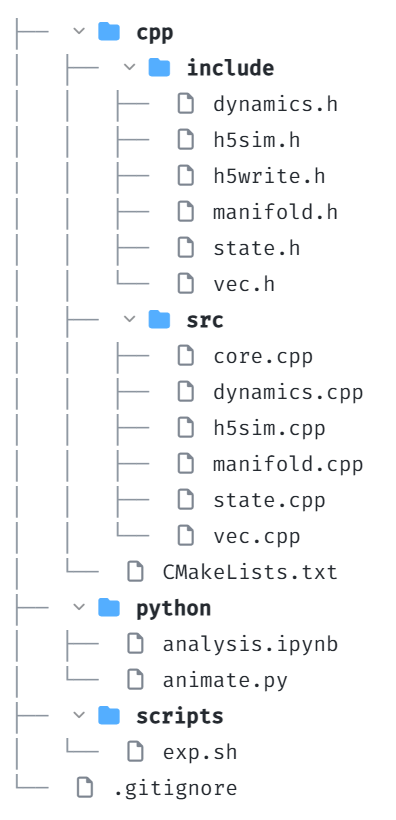
\includegraphics[width=0.8\textwidth]{figures/repo_structure.png}
        \end{figure}
    \end{minipage}
\end{frame}


\begin{frame}
    \frametitle{Specific Manifolds}

    \begin{itemize}
        \item I chose to implement a spherical and toroidal manifold,
        as well as regular Euclidean space as a control.
        \item The coordinate chart on the sphere is as usual: 
        $q_1 = \phi \in [0, 2\pi)$ (azimuthal angle),
        $q_2 = \alpha \in [0, \pi)$ (polar angle, usually $\theta$ but that's taken).
        For radius $R$, the metric is:
        \begin{align*}
            g_\text{sphere} = \begin{bmatrix}
                R^2\sin^2\alpha & 0 \\
                0 & R^2
            \end{bmatrix}
        \end{align*}
        \item The coordinate chart on the sphere is $q_1 = \phi \in [0,2\pi)$
        (toroidal angle) $q_2 = \psi \in [0,2\pi)$ (poloidal angle).
        With major radius $R$ and minor radius $r$, the metric is:
        \begin{align*}
            g_\text{torus} = \begin{bmatrix}
                (R + r\cos\psi)^2 & 0 \\
                0 & r^2
            \end{bmatrix}
        \end{align*}
    \end{itemize}
\end{frame}

\begin{frame}
    \frametitle{The Vaguest Possible Pseudocode Overview}

    \begin{algorithm}[H]
        \begin{algorithmic}[1]
        \Procedure{StepSimulation}{$\Delta t$}
            \State \textbf{Phase 1: Geometry \& Dynamics}
            \For{each particle $i$}
                \State $\theta_i \gets \theta_i + \omega + \sqrt{2D\Delta t} \cdot \mathcal{N}(0,1)$ \Comment{Update Orientation}
                \State $q_i \gets q_i + \text{Vielbein}(q_i) \cdot \vec{v}(\theta_i) \Delta t$ \Comment{Update Position}
                \State \text{Manifold.wrap}($q_i$) \Comment{Boundary conditions}
            \EndFor
            
            \State \textbf{Phase 2: Interaction \& Alignment}
            \For{each pair $(i, j)$ within $R_{int}$}
                \If{$d(i,j) < 2s_{radius}$}
                    \State \text{ResolveCollision}($i, j$) \Comment{Elastic reflection}
                \EndIf
                \State \text{ParallelTransport}($\theta_i \leftrightarrow \theta_j$) \Comment{Align tangent spaces}
                \State $\theta_i \gets \theta_i + \sum \sin(\theta_\text{mean} - \theta_i) \Delta t$ \Comment{Vicsek alignment}
            \EndFor
        \EndProcedure
        \end{algorithmic}
    \end{algorithm}

\end{frame}

\begin{frame}
    \frametitle{Investigation of the Scientific Question}

    \begin{itemize}
        \item At the beginning, I said the goal was to see how different manifolds
        exhibit different behavior.
        \item The specific behavior we're looking at is the phase-transition 
        that comes from the interplay of the diffusion and coupling coefficients.
        \item At high diffusion, the particles act like a gas, moving randomly
        and overcoming their orientational alignment.
        \item At high coupling, the particles act like a fluid, flowing in groups
        along the surface.
        \item Each ``experiment'' run consists of running the algorithm
        on the previous slide for a large number of timesteps on each
        of our three manifolds, with four different values of $C$ and $D$.
        \item By computing the global order parameter for each manifold
        over different sets of parameters, we can see how alignment
        behaves as a function of $C$, $D$, and the manifold.
        \item For fun, we also animate the particle trajectories.
    \end{itemize}
\end{frame}

% RESULTS RESULTS 
\section{Results}

\begin{frame}
    \frametitle{Global Order Parameter}

    \begin{itemize}
        \item To compare the alignment behavior across manifolds, we modify
        the typical Vicsek global order parameter:
        \begin{align*}
            \Phi = \left\langle
                \left|\frac{1}{N}\sum_i^N \mathbf{v}_i\right|
            \right\rangle
        \end{align*}
        \item It ranges from 0 to 1, with 0 being complete random alignment (gas-like behavior)
        and 1 being complete global alignment (flocking) of all particles. 
        \item $\langle \cdot \rangle$ is a time average over the end of the simulation,
        ensuring steady-state behavior rather than a transient coincidence.
        \item Particles moving in the same direction on a curved surface will
        not have the same $\mathbf{v}_i$ vector in 3D space; we must first
        parallel transport the vectors to the same location on the surface, with
        $\bar{\theta}_i$ equal to the orientation after transport.
        \begin{align*}
            \Phi_\text{intrinsic} = \left\langle
                \left|\frac{1}{N}\sum_i^N e^{i\bar{\theta}_i}\right|
            \right\rangle
        \end{align*}
    \end{itemize}
\end{frame}

\begin{frame}
    \frametitle{Global Order Parameter Results}

    \begin{figure}[h]
        \centering
        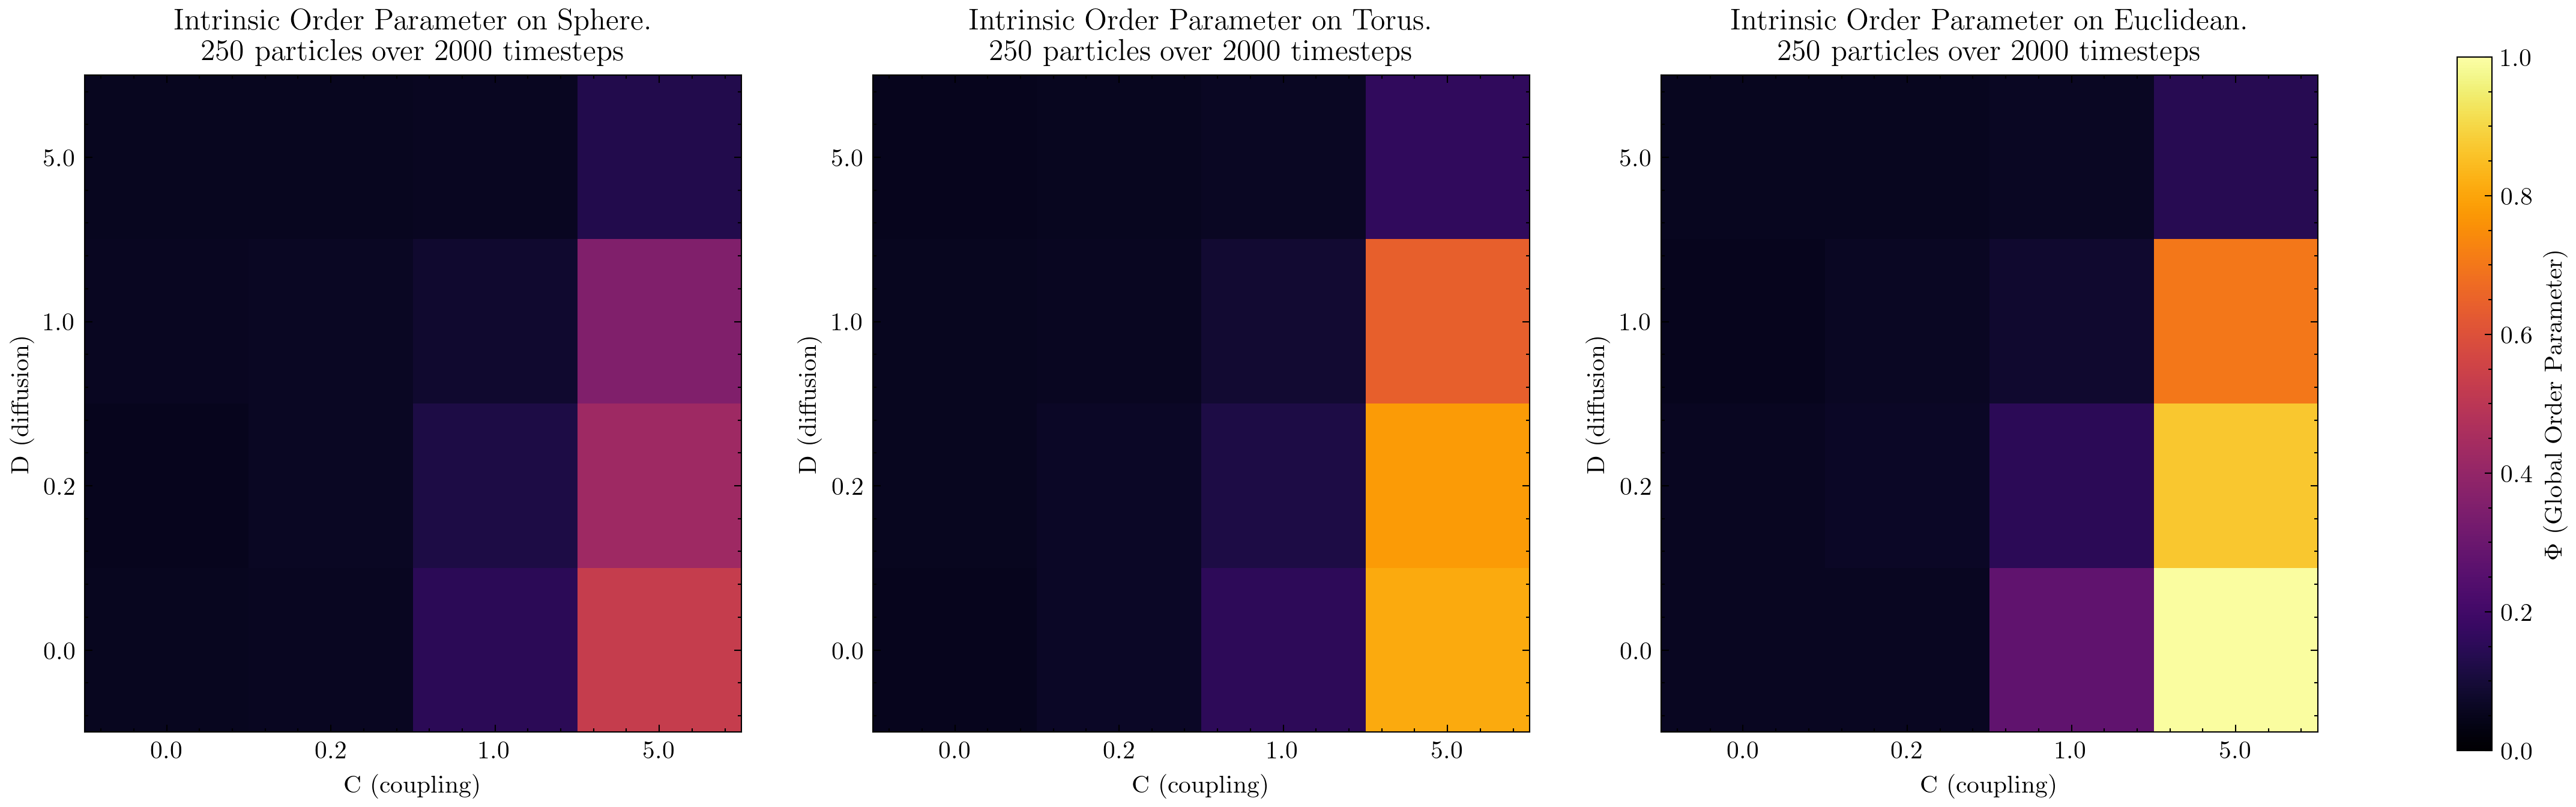
\includegraphics[width=\textwidth]{figures/int_order2.png}
    \end{figure}

    \begin{itemize}
        \item In general, we see what we expect: particles align far more
        in low diffusion, high coupling regimes.
        \item The phase transition is likely gradual; our parameter sweep
        is too restricted to see intermediate behavior.
        \item In general, curvature makes global alignment
        more difficult.
    \end{itemize}
\end{frame}


\begin{frame}
    \frametitle{Animations?}
    Embedding animations in a PDF is a pain. I've gathered
    some still preview images for completeness. Pivoting to live demonstration!
    \vspace{1.5cm}

    \begin{minipage}[c]{0.3\textwidth}
        \begin{figure}[h]
            \centering
            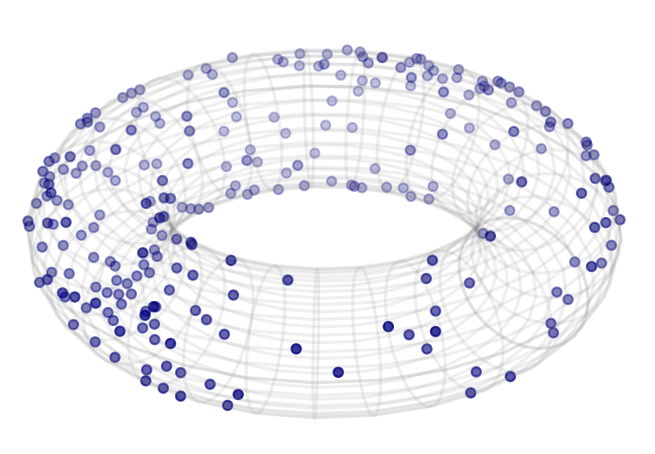
\includegraphics[width=0.8\textwidth]{figures/torus.png}
        \end{figure}
    \end{minipage}
    %
    \hfill
    %
    \begin{minipage}[c]{0.3\textwidth}
        \begin{figure}[h]
            \centering
            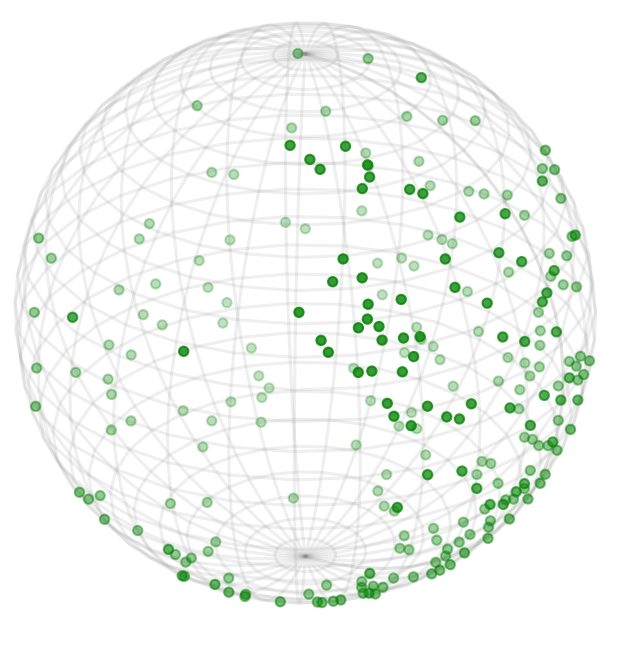
\includegraphics[width=0.8\textwidth]{figures/sphere.png}
        \end{figure}
    \end{minipage}
    %
    \hfill
    %
    \begin{minipage}[c]{0.3\textwidth}
        \begin{figure}[h]
            \centering
            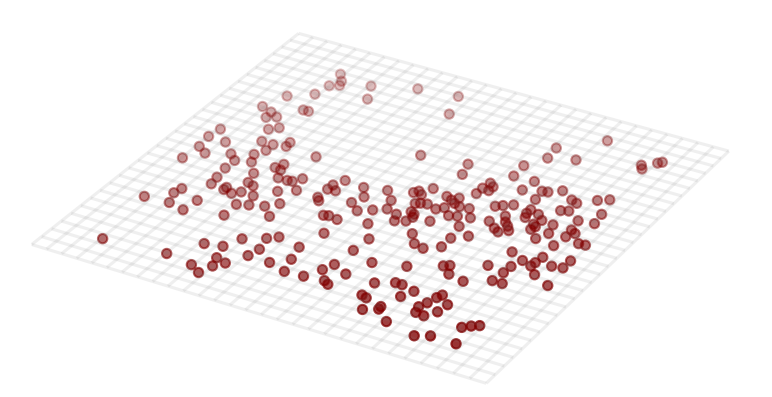
\includegraphics[width=0.8\textwidth]{figures/euclidean.png}
        \end{figure}
    \end{minipage}
    
\end{frame}



\section{Conclusion}

\begin{frame}
    \frametitle{In Conclusion}
    
    \begin{itemize}
        \item Successfully implemented a C\texttt{++}/Python pipeline for simulating interacting ABPs on arbitrary 2D Riemannian manifolds.
        \item Quantitatively demonstrated phase-transition across parameter sweeps
        for different manifolds.
        \item In general, it seems it is more difficult for particles to align
        on curved surfaces.
        \item Further testing with larger parameter sweeps, investigations
        into initial particle density, etc, will be necessary to codify this result.
    \end{itemize}
\end{frame}


\begin{frame}
    \frametitle{}
    \vfill
    \centering
    \Huge \textbf{Thank You}
    \vfill
    \Large Questions?
    \vfill
\end{frame}



\end{document}